\documentclass[12pt,a4paper]{article}
\usepackage[slovene]{babel}
\usepackage[T1]{fontenc}
\usepackage[utf8]{inputenc}
\usepackage{amsmath,amssymb,amsfonts,amsthm}
\usepackage{url}
\usepackage[dvipsnames,usenames]{color}
\usepackage{graphicx}

% mine
% \usepackage[all]{xy}  % diagrami
\usepackage{mathrsfs} % for mathscr
\usepackage{stmaryrd} % oklepaji
\usepackage[bookmarks, bookmarksopen, bookmarksdepth=3, colorlinks=true,
  linkcolor=black, anchorcolor=black, citecolor=black, filecolor=black,
  menucolor=black, runcolor=black, urlcolor=black, pdfencoding=unicode
]{hyperref}

% ne spreminjaj podatkov, ki vplivajo na obliko strani
\textwidth 15cm
\textheight 24cm
\oddsidemargin.5cm
\evensidemargin.5cm
\topmargin-5mm
\addtolength{\footskip}{10pt}
\pagestyle{plain}
\overfullrule=15pt % oznaci predlogo vrstico


% ukazi za matematicna okolja
\theoremstyle{definition} % tekst napisan pokoncno
\newtheorem{definicija}{Definicija}[section]
\newtheorem{primer}[definicija]{Primer}
\newtheorem{opomba}[definicija]{Opomba}

\theoremstyle{plain} % tekst napisan posevno
\newtheorem{lema}[definicija]{Lema}
\newtheorem{izrek}[definicija]{Izrek}
\newtheorem{trditev}[definicija]{Trditev}
\newtheorem{posledica}[definicija]{Posledica}


% za stevilske mnozice uporabi naslednje simbole
\newcommand{\R}{\mathbb R}
\newcommand{\N}{\mathbb N}
\newcommand{\Z}{\mathbb Z}
\renewcommand{\C}{\mathbb C}  % defined by xypic
\newcommand{\Q}{\mathbb Q}
\newcommand{\Rc}{\mathcal{R}}
\newcommand{\Nc}{\mathcal{N}}
\newcommand{\I}{\mathcal{I}}
\newcommand{\B}{\mathcal{B}}
\renewcommand{\L}{\mathcal{L}}
\newcommand{\T}{\mathsf{T}}

% naslednje ukaze ustrezno popravi
\newcommand{\program}{Matematika} % ime studijskega programa
\newcommand{\imeavtorja}{Jure Slak} % ime avtorja
\newcommand{\imementorja}{doc.~dr.~George Mejak} % akademski naziv in ime mentorja
\newcommand{\imesomentorja}{dr.~Gregor Kosec} % akademski naziv in ime mentorja
\newcommand{\naslovdela}{TBA}
\newcommand{\letnica}{2017} %letnica diplome

% lists with less vertical space
\newenvironment{itemize*}{\vspace{-1.5\parskip}\begin{itemize}\setlength{\itemsep}{0pt}\setlength{\parskip}{2pt}}{\end{itemize}\vspace{-1\parskip}}
\newenvironment{enumerate*}{\vspace{-1.5\parskip}\begin{enumerate}\setlength{\itemsep}{0pt}\setlength{\parskip}{2pt}}{\end{enumerate}\vspace{-1\parskip}}
\newenvironment{description*}{\vspace{-6pt}\begin{description}\setlength{\itemsep}{0pt}\setlength{\parskip}{2pt}}{\end{description}\vspace{-1\parskip}}

% vstavi svoje definicije ...
\hypersetup{pdftitle={\naslovdela}}
\hypersetup{pdfauthor={\imeavtorja}}
\hypersetup{pdfsubject={delo diplomskega seminarja}}

% matematika
\newcommand{\lap}{\operatorname{lap}}
\renewcommand{\div}{\operatorname{div}}
\newcommand{\grad}{\operatorname{grad}}
\renewcommand{\b}{\boldsymbol}
\let\oldphi\phi
\renewcommand{\phi}{\varphi}
\newcommand{\eps}{\varepsilon}
\newcommand{\zomega}{\overline{\Omega}}
\newcommand{\Lin}{\mathcal{L}in}
\newcommand{\uh}{\hat{u}}

% partial derivatives
\newcommand{\dpar}[2]{\ensuremath{\frac{\partial #1}{\partial #2}}}
\newcommand{\dpr}[1]{\dpar{#1}{r}}
\newcommand{\dpt}[1]{\dpar{#1}{t}}
\newcommand{\dpx}[1]{\dpar{#1}{x}}
\newcommand{\dpy}[1]{\dpar{#1}{y}}
\newcommand{\dpz}[1]{\dpar{#1}{z}}
\newcommand{\dpth}[1]{\dpar{#1}{\theta}}
\newcommand{\dpfi}[1]{\dpar{#1}{\varphi}}

% total derivatives
\newcommand{\dd}[2]{\ensuremath{\frac{d #1}{d #2}}}
\newcommand{\ddr}[1]{\dd{#1}{r}}
\newcommand{\ddt}[1]{\dd{#1}{t}}
\newcommand{\ddx}[1]{\dd{#1}{x}}
\newcommand{\ddy}[1]{\dd{#1}{y}}
\newcommand{\ddz}[1]{\dd{#1}{z}}
\newcommand{\ddth}[1]{\dd{#1}{\theta}}

% operators
\DeclareMathOperator{\diag}{diag}
\DeclareMathOperator{\nnz}{nnz}

% slovnica
\newcommand{\ang}[1]{\text{(\textit{angl.} #1)}}


% bold math in sections
\SetSymbolFont{stmry}{bold}{U}{stmry}{m}{n}
\makeatletter
\g@addto@macro\bfseries{\boldmath}
\makeatother

% algorithms
\usepackage{algpseudocode}
\usepackage{algorithm}

\floatname{algorithm}{Algoritem}
\algnewcommand\algorithmicto{\textbf{to}}
\algrenewtext{For}[3]{$\algorithmicfor\ #1 \gets #2\ \algorithmicto\ #3\ \algorithmicdo$}


%%%%%%%%%%%%%%%%%%%%%%%%%%%%%%%%%%%%%%%%%%%%%%%%%%%%%%%%%%%%%%%%%%%%%%%%%%%%%%%%
%%%%%%           DOCUMENT           %%%%%%%%%%%%%%%%%%%%%%%%%%%%%%%%%%%%%%%%%%%%
%%%%%%%%%%%%%%%%%%%%%%%%%%%%%%%%%%%%%%%%%%%%%%%%%%%%%%%%%%%%%%%%%%%%%%%%%%%%%%%%

\pagenumbering{roman}

\begin{document}

% od tod do povzetka ne spreminjaj nicesar
\thispagestyle{empty}
\noindent{\large
UNIVERZA V LJUBLJANI\\[1mm]
FAKULTETA ZA MATEMATIKO IN FIZIKO\\[5mm]
\program\ -- 2.~stopnja}
\vfill

\begin{center}{\large
\imeavtorja\\[2mm]
{\bf \naslovdela}\\[10mm]
Magistrsko delo \\[1cm]
Mentor: \imementorja \\[2mm]
Somentor: \imesomentorja}
\end{center}
\vfill

\noindent{\large
Ljubljana, \letnica}
\pagebreak


\tableofcontents
\pagebreak

\begin{center}
{\bf \naslovdela}\\[3mm]
{\sc Povzetek}
\end{center}
TBA
\vfill
\begin{center}
{\bf TBA}\\[3mm] % prevod slovenskega naslova dela
{\sc Abstract}
\end{center}
TBA

\vfill\noindent
{\bf Math. Subj. Class. (2010):}  \\[1mm]
{\bf Ključne besede:} ?? \\[1mm]
{\bf Keywords:} ??
\pagebreak


\setcounter{page}{1}
\pagenumbering{arabic}

\section{Uvod}

Uporabili bomo~\cite{lebedev2009introduction}.

\newpage

\section{Numerična metoda}
\label{sec:numericna-metoda}

V 20.~stoletju je skupaj z razvojem računalnikov začel svojo pot razvoj numeričnih
metod za reševaje parcialnih diferencialnih enačb. Do danes je bilo razvitih
veliko metod za numerično reševanje parcialnih diferencialnih enačb. Dva
pomembna razreda metod se ločita glede na obliko v kateri rešujemo parcialno
diferencialno enačbo: šibki~\ang{weak form} ali močni~\ang{strong form}.
Najznamenitejši in zelo uspešen predstavnik prve skupine je metoda končnih
elementov (MKE)~\ang{finite element method (FEM}, kjer problem najprej prevedemo
v šibko obliko, nato pa rešitev poiščemo kot linearno kombinacijo baznih
funkcij iz izbranega prostora. Najbolj poznan, predstavnik druge pa je metoda
končnih diferenc (MKD)~\ang{finite diference method (FDM)}, pri kateri
direktno diskretiziramo operator, ki nastopa v enačbi.

Poleg tega se metode delijo tudi, glede na tip diskretizacije domene, ki ga
potrebujejo. Metoda končnih elementov potrebuje \emph{mrežo}, nad katero deluje,
tj. triangulacijo notranjosti domene, ki inducira tudi mrežo na robu.
Metoda robnih elementov potrebuje samo mrežo na robu domene. Metoda končnih
diferenc je običajno formulirana na pravokotni mreži. Obstajajo pa tudi
metode, ki mreže ne potrebujejo, imenujemo jih \emph{brezmrežne
metode}~\ang{meshfree methods}. Predstavljena metoda v tem razdelku, bo reševala
enačbo v močni obliki in bo brezmrežna.

\subsection{Izpeljava}

Izpeljavo začnimo z osvežitvijo spomina na metodo končnih diferenc, ki nam bo
služila kot motivacija.

\subsubsection{Ideja in motivacija}

\begin{primer}
\label{prim:fdm}
Rešujemo enodimenzionalno Poissonovo enačbo. Izpeljava metode končnih diferenc
ne bo povsem običajna in tudi ne najkrajša možna, ampak bo narejena tako, da
jo bomo lahko posplošili v brezmrežno metodo.

Rešujemo problem z mešanimi robnimi pogoji
\begin{align}
  u''(x) &= f(x) \quad \text{ na } (a, b) \label{eq:example-prob} \\
  u(a) &= A \nonumber \\
  u'(b) &= B, \nonumber
\end{align}
katerega rešitev poznamo v kvadraturah
\[
  u(x) = \int_a^x\left(\int_b^\eta f(\xi) d\xi \right) d\eta + B(x-a) + A.
\]

Numeričnega reševanja se lotimo tako, da interval $[a, b]$ diskretiziramo na
$N$ enakih delov dolžine $h = \frac{b-a}{N}$ z delilnimi točkami $x_i = a + i h$, za $i = 0,
\dots, N$. Za vsako od teh točk uvedemo neznanko $u_i$, ki predstavlja
neznano funkcijsko vrednost v točki $x_i$. S pomočjo vrednosti $u_{i-1}, u_i$
in $u_{i+1}$ želimo sedaj aproksimirati $u''(x_i)$. To nam bo dalo zvezo med
spremenljivkami in ko jo uporabimo za vse notranje točke ter upoštevamo še
robne pogoje, bomo dobili sistem linearnih enačb, katerega rešitev nam bo dala
dobro aproksimacijo funkcije $u$.

Funkcijo $u$ v okolici $x_i$ aproksimiramo z interpolacijskim polinomom, njene
odvode pa z odvodi interpolacijskega polinoma. Da najdemo interpolacijski
polinom $\hat{u}$, zapišimo
\[
  \hat{u}(x) = \alpha_0 + \alpha_1x + \alpha_2x^2 =
  \begin{bmatrix}
    1 & x & x^2
  \end{bmatrix}
  \begin{bmatrix}
    \alpha_0 \\ \alpha_1 \\ \alpha_2
  \end{bmatrix} = \b{b}(x)^\T\b{\alpha}
\]
in poiščimo koeficiente $\b{\alpha}$, da bo veljalo
\begin{align*}
  \hat{u}(x_{i-1}) &= u_{i-1} \\
  \hat{u}(x_{i}) &= u_{i} \\
  \hat{u}(x_{i+1}) &= u_{i+1}.
\end{align*}
Če sistem enačb razpišemo, dobimo
\begin{align*}
  \alpha_0 + \alpha_1 (x_i -h) + \alpha_2 (x_i-h)^2 &= u_{i-1} \\
  \alpha_0 + \alpha_1 x_{i} + \alpha_2 x_{i}^2 &= u_{i} \\
  \alpha_0 + \alpha_1 (x_i +h) + \alpha_2 (x_i+h)^2 &= u_{i+1}
\end{align*}
oziroma v matrični obliki
\[
  \begin{bmatrix}
    1 & x_i - h & (x_i-h)^2 \\
    1 & x_i & x_i^2 \\
    1 & x_i + h & (x_i+h)^2
  \end{bmatrix}
  \begin{bmatrix}
    \alpha_0 \\ \alpha_1 \\ \alpha_2
  \end{bmatrix}
  =
  \begin{bmatrix}
    u_{i-1} \\ u_i  \\ u_{i+1}
  \end{bmatrix}.
\]
Krajše ga zapišemo kar kot $B\b\alpha = \b{u}$. Sistem rešimo in dobimo
\begin{align*}
  \alpha_0 &= \frac{2 h^2 u_{i}+h (u_{i-1}-u_{i+1}) x_i+(u_{i-1}-2 u_{i}+u_{i+1}) x_i^2}{2 h^2} \\
  \alpha_1 &= \frac{h (u_{i+1}-u_{i-1})-2 (u_{i-1}-2 u_{i}+u_{i+1}) x_i}{2 h^2} \\
  \alpha_2 &= \frac{u_{i-1}-2 u_{i}+u_{i+1}}{2 h^2}.
\end{align*}
Interpolacijski polinom skozi točke $(x_i, u_i)$ lahko sedaj zapišemo kot
\begin{align*}
  \hat{u}(x) &=
  \begin{bmatrix}
    1 & x & x^2
  \end{bmatrix}
  \begin{bmatrix}
    \alpha_0 \\ \alpha_1 \\ \alpha_2
  \end{bmatrix} = \\
  &= u_i +\frac{u_{i+1}-u_{i-1}}{2 h}(x-x_i)+\frac{u_{i-1}-2 u_{i}+u_{i+1}}{2 h^2}(x-x_i)^2
\end{align*}
Toda, ker $u_j$ nastopajo linearno, lahko napišemo tudi v obliki
\[
  \hat{u}(x) =
  \begin{bmatrix}
  \frac{(x_i-x) (h+x_i-x)}{2 h^2} & \frac{(h+x-x_i)(h+x_i-x)}{h^2} & \frac{(x-x_i) (h+x-x_i)}{2 h^2}
  \end{bmatrix}
  \begin{bmatrix}
    u_{i-1} \\ u_{i} \\ u_{i+1}
  \end{bmatrix}= \b\phi(x)^\T\b u.
\]
S tem smo ločili podatke, ki se nanašajo na vrednost funkcije, od podatkov, ki
se nanašajo na pozicije točk. Če na primer vemo, da bomo večkrat potrebovali
vrednost interpolacijskega polinoma v neki točki $x^\ast$ za različne nabore
funkcijskih vrednosti (vendar še vedno izmerjene v istih točkah) $\b u$, potem
se nam splača poračunati $\b\phi(x^\ast)$ vnaprej in vrednosti
interpolacijskega polinoma dobimo vsakič znova le s skalarnim produktom $\hat
u(x^\ast) = \b\phi(x^\ast) ^\T \b u$.

Za aproksimacijo $u'$ in $u''$ bomo vzeli kar odvode $\hat{u}$. Izračunajmo
jih v točki $x_i$ in dobimo znane formule
\begin{align*}
  \hat u'(x_i) &= \b\phi'(x_i)^\T \b u =
  \begin{bmatrix}
    -\frac{1}{2h} & 0 & \frac{1}{2h}
  \end{bmatrix} \begin{bmatrix}
    u_{i-1} \\ u_{i} \\ u_{i+1}
  \end{bmatrix}\\
  \hat u''(x_i) &= \b\phi''(x_i)^\T \b u =
  \begin{bmatrix}
    \frac{1}{h^2} & -\frac{2}{h^2} & \frac{1}{h^2}
  \end{bmatrix}\begin{bmatrix}
    u_{i-1} \\ u_{i} \\ u_{i+1}
  \end{bmatrix}.
\end{align*}

To lahko uporabimo za reševanje našega problema~\eqref{eq:example-prob}.
Namesto enakosti
\[ u''(x_i) = f(x_i) \]
za vsako točko $x_i$ v notranjosti naredimo zapišemo podobno enakost
\[
  \begin{bmatrix}
    \frac{1}{h^2} & -\frac{2}{h^2} & \frac{1}{h^2}
  \end{bmatrix}\begin{bmatrix}
    u_{i-1} \\ u_{i} \\ u_{i+1}
  \end{bmatrix} = f(x_i).
\]
Dirichletov pogoj na levem robu zapišemo preprosto kot $u_0 = A$,
za Neumannovega na desnem robu pa lahko uporabimo npr. enostransko diferenco
na treh točkah \[
  \begin{bmatrix}
    \frac{1}{2h} & \frac{-2}{h} & \frac{3}{2h}
  \end{bmatrix}\begin{bmatrix}
    u_{N-2} \\ u_{N-1} \\ u_{N}
  \end{bmatrix} = B,
\]
ki bi jo izpeljali na enak način.

Vse te enakosti zložimo sistem enačb in ga zapišimo v matrični obliki
\begin{align*}
  \begin{bmatrix}
    1 &  \\
    -1 & 2 & 1 \\
    & -1 & 2 & 1 \\
    & & \!\ddots & \!\ddots & \! \ddots \\
    &&& -1 & 2 & 1 \\
    &&& 1/2h & -2/h & 3/2h \\
  \end{bmatrix}
\begin{bmatrix}
  u_0 \\ u_1 \\ u_2 \\ \vdots \\ u_{N-1} \\ u_N
\end{bmatrix}
 =
 \begin{bmatrix}
   f(x_0) \\
   f(x_1) \\
   f(x_2) \\
   \vdots \\
   f(x_{N-1}) \\
   f(x_N)
 \end{bmatrix}.
\end{align*}
Rešitev tega sistema nam dobro aproksimira neznano funkcijo $u$ v izbranih
točkah $x_i$.
\end{primer}

\subsubsection{Splošna izpeljava}
\label{sec:splosna-izpeljava}
Postavimo se sedaj v splošnejši okvir.
Rešujmo parcialno diferencialno enačbo
\begin{align}
  \L u &= f \text{ na } \Omega, \label{eq:general-problem} \\
  \Rc u &= g \text{ na } \partial \Omega \nonumber,
\end{align}
kjer je $\Omega \subseteq \R^d$ omejena domena, torej, omejena povezana odprta
množica z odsekoma gladkim robom, $u \in C^r(\R^d)$ funkcija,
$\L\colon C^r(\R^d) \to C(\R)$ linearen
parcialni diferencialni operator reda $r$ in $\Rc u$ robni pogoji,
pri katerih je problem enolično rešljiv.

Domeno in njen rob sedaj diskretiziramo, tako da izberemo $N$ točk v zaprtju
domene, $x_1, \dots, x_N \in \zomega$. Podobno kot pri končnih
diferencah bomo v teh točkah aproksimirali vrednost funkcije $u$.
Izberimo fiksno točko $p \in \zomega$ in $n$ izmed točk $\{x_1, \dots, x_N\}$,
ki bodo sestavljali \emph{soseščino}~\ang{support} točke $p$. Število $n$ imenujemo
velikost soseščine. Označimo z $\Nc(p)$ soseščino točke $p$ in
z $\I(p) = \{i_1, \dots, i_n\}$ množico indeksov, za katere so izbrani
$x_{i_j}$ v soseščini $p$. Velja torej \[
  \Nc(p) = \bigcup_{i \in \I(p)} x_i.
\]
Običajno bo $n \ll N$, npr. $n = 9$ in $N = 10^6$.
Primer domene $\Omega$, točke $p$ in njene soseščine je prikazan na
sliki~\ref{fig:domain-example}.

\begin{figure}[ht]
  \centering
  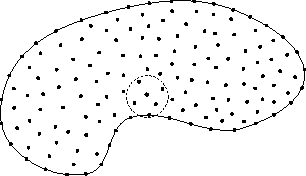
\includegraphics[width=0.7\textwidth]{images/domain_theoretical.pdf}
  \caption{Primer domene z diskretizirano notranjostjo in robom skupaj z izbrano
  točko in njeno soseščino.}
  \label{fig:domain-example}
\end{figure}

V okolici točke $p$ aproksimirajmo $u$ z elementi iz nekega končno
dimenzionalnega prostora funkcij $\B = \Lin\{b_1, \dots, b_m\}$.
Funkcijam $b_i\colon \R^d \to \R$ pravimo \emph{bazne funkcije},
številu $m$ pa moč baze. Aproksimacijo za $\uh$ za $u$ lahko torej zapišemo kot
\[
  u \approx \uh = \sum_{i=1}^m \alpha_i b_i = \b{b}^\T \b{\alpha},
\]
pri čemer smo z $\b{\alpha} = (\alpha_i)_{i=1}^m$ označili vektor neznanih
koeficientov in $\b{b} = (b_i)_{i=1}^m$ vektor baznih funkcij.

Če bi poznali vrednosti $u(x_i)$ za $i \in I(p)$, potem bi lahko aproksimiranko
$\uh$ izračunali po metodi najmanjših kvadratov. Ker pa teh vrednosti ne
poznamo, uvedimo spremenljivke $u_i$ za vsako točko v domeni, ki nam bodo
predstavljale neznane prave vrednosti in nadaljujmo
s simbolnim računanjem. Za funkcijo $\uh$ zahtevamo, da aproksimira $u$ v smislu
utežene diskretne 2-norme, torej da minimizira
\begin{align*}
  \|u-\uh\|_{2,N(p),\b{w}} &= \sum_{i\in I(p)} w(p-x_i) (u_i - \uh(x_i))^2
\end{align*}
kar je utežena vsota kvadratov odstopanj od pravih vrednosti. Pri tem je
$w\colon\R^d\to\R$ nenegativna funkcija, ki jo imenujemo \emph{utež}, $\b{w}$ pa
je vektor sestavljen iz vrednosti te funkcije v točkah v soseščini.

Matrično lahko zapišemo sistem enačb, ki po vrsticah
postavlja našo zahtevo $\hat{u}(x_j) = u_j$, za vsak $j \in I(p)$:
\[
\begin{bmatrix}
  b_1(x_{i_1}) & \cdots & b_m(x_{i_1}) \\
  \vdots & \ddots & \vdots   \\
  b_1(x_{i_n}) & \cdots & b_m(x_{i_n})
\end{bmatrix}
\begin{bmatrix}
  \alpha_1 \\ \vdots \\ \alpha_m
\end{bmatrix}
=
\begin{bmatrix}
  u_{i_1} \\ \vdots \\ u_{i_n}
\end{bmatrix}.
\]
Na krajše sistem zapišemo kot $B\b{\alpha} = \b{\tilde{u}}$. Odvisno od
$n$, $m$, $b_i$ in uteži $w$ je ta sistem lahko poddoločen, predoločen ali
običajen. V vsakem primeru lahko minimiziranje utežene napake prevedemo na
minimiziranje diskretne 2-norme $\|WB\b{\alpha}-W\b{\tilde{u}}\|_{2,N(p)}$, kjer je $W$
diagonalna matrika iz korenov uteži za posamezne točke, $W =
\diag(\sqrt{w(x_{i_1}-p)}, \dots, \sqrt{w(x_{i_n}-p)})$. Tak sistem pa lahko ne
glede na njegovo določenost v rešimo s pomočjo Moore-Penroseovega
psevdoinverza, ki ga lahko izračunamo s pomočjo singularnega razcepa matrike
$WB$.
Tako lahko izrazimo \[ \b{\alpha} = (WB)^{+}W\b{\tilde u}, \]
kjer $+$ označuje Moore-Penroseov psevdoinverz.

To lahko vstavimo nazaj v izraz za $\hat{u}$ in dobimo
\[
  \hat{u} = \b{b}^\T\b{\alpha} = \b{b}^\T(WB)^{+}W\b{\tilde{u}}.
\]
Sedaj lahko za izbrano točko $p$ izračunamo
\[
  \hat{u}(p) = \underbrace{\b{b}(p)^\T(WB)^{+}W}_{\b\phi_p}\b{\tilde{u}}.
\]
Izračunljivi kos $\b\phi_p$ je v praksi vrstica velikosti $n$, matematično pa je
linearen funkcional $\b\phi_p \in (\R^n)^\ast$, ki naboru funkcijskih vrednosti v
soseščini $N(p)$ priredi aproksimacijo za funkcijsko vrednost v točki $p$.

Podobno kot pri deljenih diferencah odvode funkcije $u$ aproksimiramo z odvodi
aproksimacijskega polinoma skozi točke v soseščini, bomo tudi v našem primeru
aproksimirali odvode funkcije $u$ z odvodi $\uh$,
\[
  (\L u)(p) \approx (\L \uh)(p) = (\L\b{b})(p)^\T(WB)^{+}W \b{\tilde{u}}
\]
od koder kot prej definiramo
\begin{equation}
  \b\phi_{\L,p} = (\L\b{b})(p)^\T(WB)^{+}W
  \label{eq:shape-definition}
\end{equation}
Funkcional $\b\phi_{\L,p}$ je aproksimacija operatorja $\L$ v točki $p$.
Pogosto se ga imenuje tudi \emph{funkcija oblike}~\ang{shape function}, saj v
sebi nosi podatke o lokalni obliki domene in izboru okoliških točk, ter seveda o
obnašanju $\L$ v tej okolici. Tudi če funkcijskih vrednosti $\b{\tilde{u}}$ v
okolici $p$ ne poznamo, lahko $\b\phi_{\L, p}$ izračunamo in kasneje samo s
skalarnim produktom dobimo aproksimacijo za $(\L u)(p)$. Lahko pa to izkoristimo
za zapis linearne enačbe
\[
  \b\phi_{\L,p} \cdot \b{\tilde{u}} = f(p),
\]
ki je direktna aproksimacija diferencialne enačbe~\eqref{eq:general-problem} v točki
$p$,
\[
  (\L u)(p) = f(p).
\]
To lahko sedaj storimo za vsako diskretizacijsko točko $x_i$ v domeni in
dobimo sistem enačb
\begin{align*}
  \b\phi_{\L,x_i} \cdot \b{\tilde{u}} &= f(x_i), \text{ za vsak $i$, tak da je $x_i \in \Omega$ } \\
  \b\phi_{\Rc,x_i} \cdot \b{\tilde{u}} &= g(x_i), \text{ za vsak $i$, tak da je $x_i \in \partial\Omega$.}
\end{align*}
Te enačbe lahko zapišemo v matrični sistem
\begin{equation}
  A\b{u} = \b{f},
  \label{eq:discretized-system}
\end{equation}
kjer ima matrika $A$ v vrsticah zapisane funkcionale $\b\phi_{\L,x_i}$, tako da so
neničelni elementi na tistih mestih, ki se pomnožijo z neznankami, ki ustrezajo
sosedom $x_i$. Natančneje, elementi matrike $A$ so
\begin{align*}
  A(k, i_j) &= \b\phi_{\L,p}(j), \text{ za vsak $k$, tak da je $x_k \in \Omega$
  in za vsak $i_j \in \I(x_k)$,} \\
  A(k, i_j) &= \b\phi_{\Rc,p}(j), \text{ za vsak $k$, tak da je $x_k \in
  \partial\Omega$ in za vsak $i_j \in \I(x_k)$.}
\end{align*}
Razumljivejša je morda kar Matlab-ova notacija
\[
A(k, I(x_k)) = \begin{cases}
    \b\phi_{\L, p} & x_k \in \Omega \\
    \b\phi_{\Rc, p} & x_k \in \partial\Omega \\
  \end{cases}, \text{ za $k = 1, \ldots, N$}.
\]
Vektor $\b{u} = (u_i)_{i=1}^N$ je vektor neznanih funkcijskih vrednosti, ki ga
iščemo, v vektorju $\b{f}$ pa so zapisani robni pogoji
\[
  \b f(k) = \begin{cases}
    f(x_k) & x_k \in \Omega \\
    g(x_k) & x_k \in \partial\Omega \\
  \end{cases}, \text{ za $k = 1, \ldots, N$}.
\]
Vidimo, da je matrika $A$ razpršena. Sama je dimenzij $N\times N$,
v vsaki vrstici pa ima največ $n$ neničelnih
elementov, torej je skupno število neničelnih elementov
\[
  \nnz(A) \leq nN.
\]
Enakost je lahko dosežena, lahko pa je tudi stroga, saj so kakšni koeficienti v $\phi_{\L,x_i}$ lahko
tudi 0, kot se to zgodi pri Dirichletovih robnih pogojih.

Sistem~\eqref{eq:discretized-system} nato rešimo in za aproksimacijo $u(x_i)$
vzamemo $u(x_i) \approx u_i$.

\subsection{Posebni primeri}
\label{sec:posebni-primeri}

\subsection{Algoritem}
V izpeljavi metode v razdelku~\ref{sec:splosna-izpeljava} je veliko detajlov
ostalo neizdelanih, kot na primer, kako diskretiziramo domeno ali kako poiščemo
sosede. Ti detajli so opisani v podrazdelkih, celotno metodo pa podajamo v
psevdokodi kot algoritem~\ref{alg:metoda}.

\begin{algorithm}[!ht]
  \caption{Brezmrežna metoda za reševanje PDE iz
  razdelka~\ref{sec:splosna-izpeljava}.}
  \textbf{Vhod:} Parcialna diferencialna enačba, kot opisana
  v~\eqref{eq:general-problem}. Parametri metode: \\
  \newcommand{\listbullet}{\hspace*{10pt}$\bullet$\hspace*{-5pt}}
  \begin{tabular}{llll}
    \listbullet & $N$     & \ldots & celotno število diskretizacijskih točk    \\
    \listbullet & $Q$     & \ldots & število diskretizacijskih točk v
    notranjosti $\Omega$ \\
    \listbullet & $n$     & \ldots & število sosedov, ki jih ima vsaka točka   \\
    \listbullet & $m$     & \ldots & število baznih funkcij                    \\
    \listbullet & $b$ & \ldots & seznam baznih funkcij dolžine $m$         \\
    \listbullet & $w$     & \ldots & utež
  \end{tabular} \\
  \textbf{Izhod:} skalarno polje $u$, ki aproksimira rešitev
  enačbe~\eqref{eq:general-problem}.
  \label{alg:metoda}
  \begin{algorithmic}[1]
    \Function{solve}{$\Omega, \L, f, \Rc, g, N, Q, n, m, b, w$}
    \State $x \gets \textsc{diskretiziraj}(\Omega, N, Q)$
    \Comment{$x$ postane seznam $N$ točk, brez škode za splošnost naj leži prvih
    $Q$ točk v $\Omega$ in preostalih $N-Q$ na $\partial \Omega$.}
    \State $s \gets $ \textsc{sosedi}$(x, n)$
    \Comment{$s$ je seznam dolžine $N$, pri čemer je $s[i]$ seznam indeksov
    elementov v $x$, ki so sosedi $x[i]$, vključno z $i$.}
    \State $\phi \gets$ prazen seznam dolžine $N$.
    \For{i}{1}{Q} \Comment{Izračunamo funkcije oblik v notranjosti.}
    \State $\phi[i] \gets$ \textsc{funkcijaOblike}$(\L, x[i], x, s[i], n, m, b, w)$
    \Comment{Glej algoritem~\ref{alg:shape-function}.}
    \EndFor
    \For{i}{Q+1}{N} \Comment{Izračunamo funkcije oblik na robu.}
    \State $\phi[i] \gets$ \textsc{funkcijaOblike}$(\Rc, x[i], x, s[i], n, m, b,
    w)$
    \Comment{Glej algoritem~\ref{alg:shape-function}.}
    \EndFor
    \State $A \gets$ prazna razpršena $N\times N$ matrika
    \For{i}{1}{N} \Comment{Aproksimiramo enačbo.}
    \For{j}{1}{n}
    \State $A[i, s[j]] \gets \phi[i][j]$
    \EndFor
    \EndFor
    \State $r \gets$ prazen vektor dolžine $N$
    \For{i}{1}{Q} \Comment{Izračunamo desno stran v notranjosti.}
    \State $r[i] \gets f(x[i])$
    \EndFor
    \For{i}{Q+1}{N} \Comment{Izračunamo robne pogoje.}
    \State $r[i] \gets g(x[i])$
    \EndFor
    \State $u \gets$ \textsc{rešiRazpršenSistem}$(A, r)$
    \State \Return $u$
    \EndFunction
  \end{algorithmic}
\end{algorithm}

\begin{algorithm}[!ht]
  \caption{Izračun funkcije oblike.}
  \textbf{Vhod:} \\
  \newcommand{\listbullet}{\hspace*{10pt}$\bullet$\hspace*{-5pt}}
  \begin{tabular}{llll}
    \listbullet & $\L$    & \ldots & parcialen diferencialen operator \\
    \listbullet & $p$     & \ldots & točka, v kateri aproksimiramo operator \\
    \listbullet & $x$     & \ldots & seznam diskretizacijskih točk \\
    \listbullet & $I$     & \ldots & množica indeksov točk v soseščini $p$ \\
    \listbullet & $n$     & \ldots & število sosedov, ki jih ima vsaka točka   \\
    \listbullet & $m$     & \ldots & število baznih funkcij                    \\
    \listbullet & $b$     & \ldots & seznam baznih funkcij dolžine $m$         \\
    \listbullet & $w$     & \ldots & utež
  \end{tabular} \\
  \textbf{Izhod:} Funkcional, ki aproksimira operator $\L$ v točki $p$.
  \label{alg:shape-function}
  \begin{algorithmic}[1]
    \Function{funkcijaOblike}{$\L, p, x, I, n, m, b, w$}
    \State $W \gets$ prazen vektor dolžine $n$
    \For{i}{1}{n}
    \State $W[i] \gets \sqrt{w(x[I[i]]-p)}$
    \EndFor
    \State $B \gets $ prazna matrika velikosti $n \times m$
    \For{i}{1}{n}
    \For{j}{1}{m}
    \State $B[i, j] \gets W[i] \cdot  b[j](x[I[i]])$
    \EndFor
    \EndFor
    \State $\ell \gets$ prazen vektor dolžine $m$
    \For{j}{1}{m}
    \State $\ell[j] \gets (\L (b[j]))(p)$
    \EndFor
    \State $\phi \gets (\ell \cdot \textsc{pinv}(B)) \cdot W$
    \Comment{Direktna analogija enačbe~\eqref{eq:shape-definition}.}
    \State \Return $\phi$
    \EndFunction
  \end{algorithmic}
\end{algorithm}

\subsubsection{Diskretizacija}
Splošno $d$-dimenzionalno domeno $\Omega$ je težko dobro diskretizirati.
Želimo si, da bi bile točke v domeni čim bolj enakomerno razporejene, saj to
pomeni, da smo dobro popisali celotno področje in upamo, da s tem tudi obnašanje
funkcije $u$, hrakti pa si zaradi numerične stabilnosti ne želimo, da bi bile
točke preveč skupaj. Uvedimo dve količini, ki nam merita ti dve lastnosti.
Za dano domeno $\Omega$ in množico točk $X$ definirajmo
\begin{align*}
  h_\Omega(X) &= \max_{p \in \Omega} \min_{x \in X} \|p - x\| \\
  S(X) &= \min_{\substack{x, y \in \Omega \\ x \neq y}} \|x-y\|
\end{align*}
Količina $h$ pove, da ne glede na to, kje v domeni smo, imamo na razdalji manj ali enako $h$
vsaj eno diskretizacijsko točko. Količina $S$ pa pove, kako blizu so si
diskretizacijske točke med seboj. Dobra diskretizacija želi maksimizirati $S$ in
minimizirati~$h$.

Algoritmi za diskretizacijo odvisni od načina, kako podamo domeno.
V našem se izkaže, da je za trenutne potrebe dovolj, da podpiramo
kvadre in krogle do vključno treh dimenzij, kot tudi unije in razlike
osnovnih oblik.

Tako lahko za diskretizacijo kvadra uporabimo kar enakomerno diskretizacijo.
Prav tako ni težko ugotoviti, kdaj so točke na robu. Za čimbolj enakomerno
diskretizacijo notranjosti kroga ali površine sfere
lahko uporabimo npr.~Fibonaccijevo mrežo, kot predlagano
v~\cite{hannay2004fibonacci} ali~v~\cite{gonzalez2010measurement}.
Pri razlikah domen preprosto izbrišemo točke, ki so padle izven domene,
pri unijah pa naredimo tudi unijo diskretizacij. Pri tem lahko potem naredimo še
en korak in pobrišemo ven kakšno izmed točk, ki so si preblizu skupaj.

Pri enakomerni diskretizaciji smo močno uporabili naše znanje o domeni in njeni
obliki. Lahko pa, da tega nimamo na voljo in želimo splošnejši algoritem, ki
potrebuje npr.~samo karakteristično funkcijo domene in njene meje, torej, kakšen
kvader, ki našo domeno vsebuje.
V tem primeru lahko vzamemo enakomerno diskretizacijo kvadra in odstranimo vse
točke, ki niso v domeni, vendar je tu težko kontrolirati število točk.
Druga metoda je, da naključno izbiramo točke v kvadru, in sprejmemo tiste, ki
pristanejo v notranjosti. Še boljšo diskretizacijo dobimo, če namesto
psevdonaključnih števil uporabimo kvazinaključna števila, ki imajo manjšo
diskrepanco. Več o tem si bralec lahko prebere v~\cite{morokoff1994quasi}.

Primeri domen in njihovih diskretizacij so prikazani na sliki~\ref{fig:domains}.

\begin{figure}[ht]
  \centering
  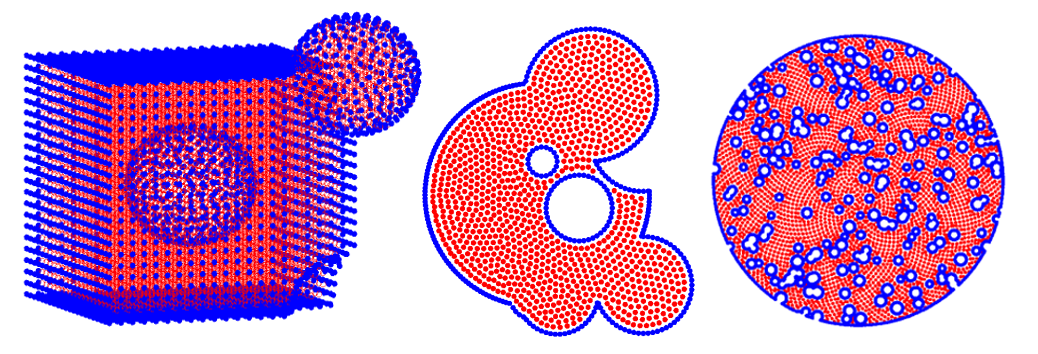
\includegraphics[width=\textwidth]{images/domains_generated.png}
  \caption{Primeri domen in njihovih diskretizacij.}
  \label{fig:domains}
\end{figure}

% relax --

\subsubsection{Iskanje najbližjih sosedov}

\subsubsection{Časovna zahtevnost}

\clearpage

\bibliographystyle{unsrt}
\bibliography{reference}

\end{document}

% vim: set spell spelllang=sl:
